\documentclass{article}
\usepackage{graphicx} % Required for inserting images
\usepackage{amsmath}
\usepackage{amssymb}
\usepackage[hidelinks]{hyperref}
\usepackage{tikz}
\usepackage{wrapfig}
\usetikzlibrary{arrows}
\usetikzlibrary{automata}
\usepackage{multicol}
\usetikzlibrary{positioning}
\usepackage[a4paper, margin=0.5in]{geometry}

\title{CSE 105 Review}
\author{Kevin Jacob}
\date{Winter 2025}

\begin{document}

\maketitle
\newpage
\section*{Table Of Contents}
\begin{enumerate}
    \item \hyperref[sec:regExpression]{Regular Expressions}
    \item \hyperref[sec:finiteAutomata]{Finite Automata}
    \item \hyperref[sec:nondeterministicAutomata]{Nondeterministic Automata}
    \item \hyperref[sec:automataConstruct]{Automata Constructions}
    \item \hyperref[sec:regLanguage]{Regular Languages}
    \item \hyperref[sec:pumpLemma]{Pumping Lemma}
    \item \hyperref[sec:proveNonregular]{Proving Nonregularity}
    \item \hyperref[sec:pushdown]{Pushdown Automata}
    \item \hyperref[sec:contextFree]{Context-free Grammars and Languages}
    \item \hyperref[sec:langClose]{Language Closures}
    \item \hyperref[sec:turing]{Turing Machines}
    \item \hyperref[sec:decide]{Recognizable and Decidable Languages}
    \item \hyperref[sec:general]{General Constructions with Turing Machines}
    \item \hyperref[sec:problems]{Computation Problems}
    \item \hyperref[sec:reduction]{Computable Functions and Mapping Reduction}
    \item \hyperref[sec:otherModels]{Other Models of Computation}
\end{enumerate}
\newpage
\section{Regular Expressions}
\label{sec:regExpression}
\subsection{Definition}
\textit{Basis steps of recursive definition}
\begin{itemize}
    \item $a$ is a regular expression, for $a\in\Sigma$
    \item $\epsilon$ is a regular expression
    \item $\emptyset$ is a regular expression
\end{itemize}
\textit{Recursive steps of recursive definition}
\begin{itemize}
    \item $(R_1\cup R_2)$ is a regular expression when $R_1,R_2$ are regular expressions\\
    $L((R_1\cup R_2))=L(R_1)\cup L(R_2)=\{w\vert w\in L(R_1) \vee w\in L(R_2)\}$
    \item $(R_1\circ R_2)$ is a regular expression when $R_1,R_2$ are regular expressions\\
    $L((R_1\circ R_2))=L(R_1)\circ L(R_2)=\{uv\vert u\in L(R_1) \wedge v\in L(R_2)\}$
    \item $R_1^*$ is a regular expression when $R_1$ is a regular expression\\
    $L((R_2)^*)=(L(R_1))^*=\{w_1,\dots,w_k\vert k\geq 0 \text{ and each } w_i\in L(R_1)\}$
\end{itemize}
\subsection{Conventions}
\textit{Assuming $\Sigma$ is the alphabet, we use the following conventions}
\begin{itemize}
    \item $\Sigma$\\
    regular expression describing language consisting of all strings of length 1 over $\Sigma$
    \item $*$ then $\circ$ then $\cup$\\
    precedence order, unless parentheses are used to change it
    \item $R_1R_2$\\
    shorthand for $R_1\circ R_2$ (concatenation symbol is implicit)
    \item $R^+$\\
    shorthand for $R^*\circ R$
    \item $R^k$\\
    shorthand for $R$ concatenated with itself $k$ times, where $k$ is a (specific) natural number
\end{itemize}
\section{Finite Automata}
\label{sec:finiteAutomata}
\subsection{Definition}
The \textbf{formal definition} of a finite automata consists of a 5-tuple $M=(Q,\Sigma,\delta,q_0,F)$ and a finite automata can also be represented by a state diagram
\begin{itemize}
\item \textbf{Finite set of states $Q$} can be labeled by any collection of distinct names
\item The \textbf{alphabet $\Sigma$} determines the possible inputs to the automaton. Each input to the automaton is a string over $\Sigma$
\item The \textbf{transition function $\delta$} gives the next state of the automaton based on the current state of the machine and on the next input symbol
\item The \textbf{start state $q_0$} is an element of $Q$. each computation of the machine starts at the start state.
\item The \textbf{accept (final) states $F$} form a subset of the states of the automaton, $F\subseteq Q$. These states flag if a machine accepts or rejects an input string.
\end{itemize}
The computation of a machine on an input string is a sequence of states in the machine, starting with the start state, determined by transitions of the machine as it reads successive input symbols.\\
\newline
The finite automaton $M$ accepts the given input string exactly when the computation of $M$ on the input string ends in an accept state.\\
\newline
The language of $M$, $L(M)$, is defined as the set of all strings that are each accepted by the machine $M$. Each string that is rejected by $M$ is not in $L(M)$.
\subsection{Example}
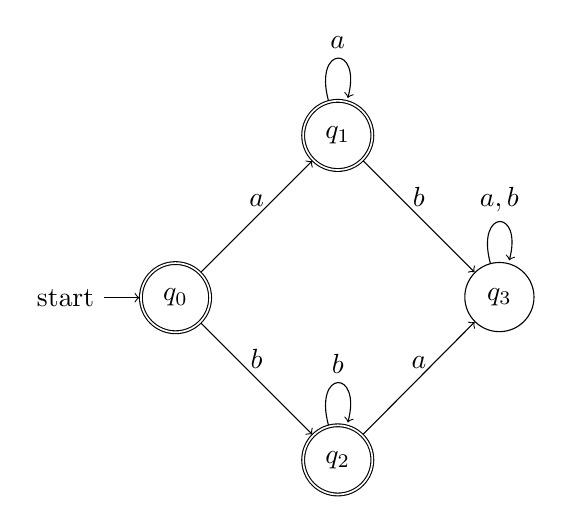
\begin{tikzpicture}[node distance=20 mm]
    \node [state,initial,accepting] (0) {$q_0$};
    \node [state,accepting] (1) [above right=of 0] {$q_1$};
    \node [state,accepting] (2) [below right=of 0] {$q_2$};
    \node [state] (3) [below right=of 1] {$q_3$};
    \path[->]
        (0) edge [above] node [align=center] {$a$} (1)
        (0) edge [above] node [align=center] {$b$} (2)
        (1) edge [loop above] node [align=center] {$a$} (1)
        (2) edge [loop above] node [align=center] {$b$} (2)
        (1) edge [above] node [align=center] {$b$} (3)
        (2) edge [above] node [align=center] {$a$} (3)
        (3) edge [loop above] node [align=center] {$a,b$} (3);
\end{tikzpicture}\\
\textbf{Formal Definition:} $(\{q_0,q_1,q_2,q_3\},\{a,b\},\delta,q_0,\{q_0,q_1,Q_2\})$\\
where $\delta: Q\times\Sigma\rightarrow Q$\\
\begin{tabular}{c|c|c}
    $Q/\Sigma$ & a & b \\
    \hline
    $q_0$ & $q_1$ & $q_2$\\
    $q_1$ & $q_1$ & $q_3$\\
    $q_2$ & $q_3$ & $q_2$\\
    $q_3$ & $q_3$ & $q_3$
\end{tabular}\\
\textbf{Language recognized by automaton:} $L(a^*\cup b^*)$
\section{Nondeterministic Automata}
\label{sec:nondeterministicAutomata}
\subsection{Definition}
The computation of a \textbf{determinstic} finite automaton has exactly one choice for its next step given the current state and character read, but an NFA allows us to have multiple\\
\newline
The \textbf{formal definition} of a nondeterministic finite automaton also consists of a 5-tuple $M=(Q,\Sigma,\delta,q_0,F)$ that can also be represented by a state diagram
\begin{itemize}
    \item \textbf{Finite set of states $Q$} can be labelled by any collection of distinct names
    \item The \textbf{alphabet $\Sigma$} where each input to the automaton is a string over $\Sigma$
    \item The \textbf{transition function $\delta:Q\times \Sigma_\epsilon\rightarrow\mathcal{P}(Q)$} gives the \textbf{set of possible next states} for a transition from the current state upon reading a symbol or spontaneously moving
    \item The \textbf{start state $q_0$} is an element of $Q$. each computation of the machine starts at the start state.
    \item The \textbf{accept (final) states $F$} form a subset of the states of the automaton, $F\subseteq Q$. These states flag if a machine accepts or rejects an input string.
\end{itemize}
$M$ accepts the input string $w\in\Sigma^*$ if and only if \textbf{there} is a computation of $M$ on $w$ that processes the \textbf{whole string} and ends in an accept state
\subsection{Example}
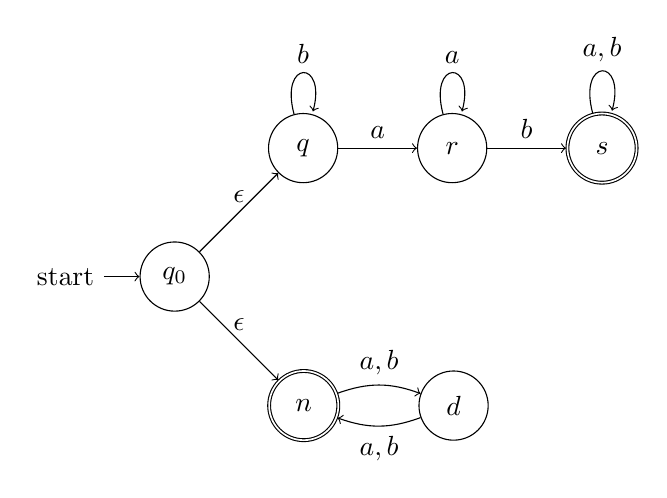
\begin{tikzpicture}
    \node [state,initial] (0) {$q_0$};
    \node [state] (1) [above right=of 0] {$q$};
    \node [state] (2) [right=of 1] {$r$};
    \node [state,accepting] (3) [right=of 2] {$s$};
    \node [state,accepting] (4) [below right=of 0] {$n$};
    \node [state] (5) [right=of 4] {$d$};
    \path[->]
        (0) edge [above] node [align=center] {$\epsilon$} (1)
        (1) edge [loop above] node [align=center] {$b$} (1)
        (1) edge [above] node [align=center] {$a$} (2)
        (2) edge [loop above] node [align=center] {$a$} (2)
        (2) edge [above] node [align=center] {$b$} (3)
        (3) edge [loop above] node [align=center] {$a,b$} (3)
        (0) edge [above] node [align=center] {$\epsilon$} (4)
        (4) edge [bend left=20] [above] node [align=center] {$a,b$} (5)
        (5) edge [bend left=20] [below] node [align=center] {$a,b$} (4);
\end{tikzpicture}\\
\textbf{Formal Definition:} $(\{q_0,q,r,s,n,d\},\{a,b\},\delta,q_0,\{s,n\})$\\
where $\delta:Q\times\Sigma_\epsilon\rightarrow\mathcal{P}(Q)$\\
\begin{tabular}{c|c|c|c}
   states/labels  & a & b & $\epsilon$ \\
   \hline
    $q_0$ & $\emptyset$ & $\emptyset$ & $\{q,n\}$\\
    $q$ & $\{r\}$ & $\{q\}$ & $\emptyset$\\
    $r$ & $\{r\}$ & $\{s\}$ & $\emptyset$\\
    $s$ & $\{s\}$ & $\{s\}$ & $\emptyset$\\
    $n$ & $\{d\}$ & $\{d\}$ & $\emptyset$\\
    $d$ & $\{n\}$ & $\{n\}$ & $\emptyset$
\end{tabular}\\
\textbf{Language recongized by NFA:} $\{w\in\{a,b\}^*\vert w \text{ has even length or has $ab$ as a substring}\}$
\section{Automata Constructions}
\label{sec:automataConstruct}
\subsection{Complementation}
\begin{itemize}
    \item The collection of languages that are each recognizable by a DFA is \textbf{closed} under complementation. We can flip the accept status of states in a DFA.
    \item The complementation construction doesn't work with an NFA\\
    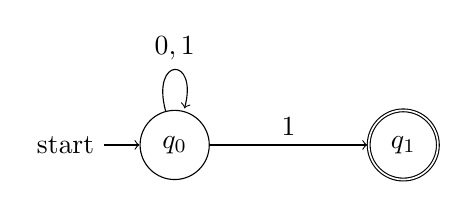
\begin{tikzpicture}[node distance=20 mm]
        \node [state,initial] (0) {$q_0$};
        \node [state,accepting] (1) [right=of 0] {$q_1$};
        \path[->]
            (0) edge [above] node [align=center] {$1$} (1)
            (0) edge [loop above] node [align=center] {$0,1$} (0);
    \end{tikzpicture}
    \hspace*{1in}
    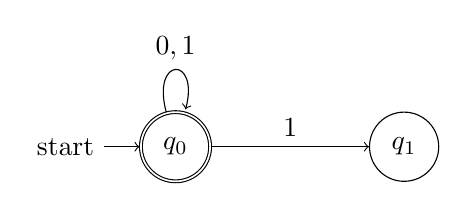
\begin{tikzpicture}[node distance=20 mm]
        \node [state,initial,accepting] (0) {$q_0$};
        \node [state] (1) [right=of 0] {$q_1$};
        \path[->]
            (0) edge [above] node [align=center] {$1$} (1)
            (0) edge [loop above] node [align=center] {$0,1$} (0);
    \end{tikzpicture}\\
    \textit{The string $1$ is accepted by both NFAs}
\end{itemize}
\subsection{Union}
\begin{itemize}
    \item The collection of languages that are each recognizable by a NFA is \textbf{closed} under union. We can add a start state and add transitions of the empty string to the start of different NFAs.
    \item We can't do the same construction since spontaneous moves are not possible in a DFA
\end{itemize}
\newpage
\subsection{DFA Constructions for Union and Intersection}
\subsubsection{Union}
Suppose $A_1,A_2$ are languages over the alphabet $\Sigma$. If there is a DFA $M_1$ such that $L(M_1)=A_1$ and a DFA $M_2$ such that $L(M_2)=A_2$, then there is a DFA $M$ such that $L(M)=A_1\cup A_2$.\\
\textbf{Formal Construction}\\
$M_1=(Q_1,\Sigma,\delta_1,q_1,F_1)$ and $M_2=(Q_2,\Sigma,\delta_2,q_2,F_2)$ where $L(M_1)=A_1$ and $L(M_2)=A_2$. We want to build $M$ with $L(M)=A_1\cup A_2$.\\
$M=(Q,\Sigma,\delta,q_0,F)$\\
$Q=\{(q,q')\vert q\in Q_1 \text{ and } q'\in Q_2\}=Q_1\times Q_2$\\
$\delta:Q\times\Sigma\rightarrow Q$\hspace*{0.5in}$\delta(((q,q'),x))=(\delta_1(q,x),\delta_2(q',x))$\\
$q_0=(q_1,q_2)$\\
$F=(F_1\times Q_2)\cup(Q_1\times F_2)$
\subsubsection{Intersection}
Suppose $A_1,A_2$ are languages over an alphabet $\Sigma$. If there is a DFA $M_1$ such that $L(M_1)=A_1$ and a DFA $M_2$ such that $L(M_2)=A_2$, then there is a DFA $M$ such that $L(M)=A_1\cap A_2$\\
\textbf{Formal Construction:}\\
$M_1=(Q_1,\Sigma,\delta_1,q_1,F_1)$ and $M_2=(Q_2,\Sigma,\delta_2,q_2,F_2)$ where $L(M_1)=A_1$ and $L(M_2)=A_2$. We want to build $M$ with $L(M)=A_1\cap A_2$.\\
$M=(Q,\Sigma,\delta,q_0,F)$\\
$Q=\{(q,q')\vert q\in Q_1 \text{ and } q'\in Q_2\}=Q_1\times Q_2$\\
$\delta:Q\times\Sigma\rightarrow Q$\hspace*{0.5in}$\delta(((q,q'),x))=(\delta_1(q,x),\delta_2(q',x))$\\
$q_0=(q_1,q_2)$\\
$F=F_1\times F_2$
\section{Regular Languages}
\label{sec:regLanguage}
If a language is regular
\begin{itemize}
    \item there is a regular expression that describes it
    \item there is a DFA that recognizes it
    \item there is a NFA that recognizes it
\end{itemize}
\subsection{Concactenation}
Suppose $A_1,A_2$ are languages over an alphabet $\Sigma$, If there is a NFA $N_1$ such that $L(N_1)=A_1$ and NFA $N_2$ such that $L(N_2)=A_2$, then there is another NFA $N$ such that $L(N)=A_1\circ A_2$\\
\textbf{Formal Construction}\\
$N_1=(Q_1,\Sigma,\delta_1,q_1,F_1)$ and $N_2=(Q_2,\Sigma,\delta_2,q_2,F_2)$ where $L(N_1)=A_1$ and $L(N_2)=A_2$. We want to build $N$ with $L(N)=A_1\circ A_2$.\\
$N=(Q,\Sigma,\delta,q_0,F)$\\
$Q=Q_1\cup Q_2$\\
$q_0=q_1$\\
$F=F_2$\\
$\delta:Q\times\Sigma_\epsilon\rightarrow\mathcal{P}(Q)$\\
$\delta((q,a))=\begin{cases}
    \delta_1((q,a))&q\in Q_1\text{ and } q\notin F_1\\
    \delta_1((q,a))&q\in F_1\text{ and }a\in\Sigma\\
    \delta_1((q,a))\cup\{q_2\}&q\in F_1\text{ and }a=\epsilon\\
    \delta_2((q,a))&q\in Q_2
\end{cases}$
\newpage
\subsection{Kleene Star}
Suppose $A$ is a language over alphabet $\Sigma$. If there is a NFA $N$ such that $L(N)=A$, then there is another NFA $N'$ such that $L(N')=A^*$.\\
\textbf{Formal Construction}\\
$N=(Q,\Sigma,\delta,q_1,F)$ where $q_0\notin Q$. We want to build $N'$ with $L(N')=A^*$.\\
$N'=(Q',\Sigma,\delta',q_0,F')$\\
$Q'=Q\cup \{q_0\}$\\
$F'=F\cup\{q_0\}$\\
$\delta':Q'\times\Sigma_\epsilon\rightarrow\mathcal{P}(Q')$\\
$\delta'((q,a))=\begin{cases}
    \delta((q,a))&q\in Q\text{ and }q\notin F\\
    \delta((q,a))&q\in F\text{ and }a\in\Sigma\\
    \delta((q,a))\cup\{q_1\}&q\in F\text{ and }a=\epsilon\\
    \{q_1\}&q=q_0\text{ and }a=\epsilon\\
    \emptyset&q=q_0\text{ and }a\in\Sigma
\end{cases}$
\subsection{NFA to DFA}
Suppose $A$ is a language over alphabet $\Sigma$. If there is a NFA $N$ such that $L(N)=A$ then there is a DFA $M$ such that $L(M)=A$\\
\textbf{Formal Construction}\\
\textit{We can treat states in $M$ as macro-states which are collections of states from $N$ that represent the set of possible states a computation of $N$ might be in.}\\
Let $N=(Q,\Sigma,\delta,q_0,F)$. We want to build $M$ with $L(M)=A$.\\
$M=(\mathcal{P}(Q),\Sigma,\delta',q',\{X\subseteq Q\vert X\cap F\neq\emptyset\})$\\
$q'=\{q\in Q\vert q=q_0\text{ or is accessible from }q_0\text{ by spontaneous moves in }N\}$\\
$\delta'((X,x))=\{q\in\delta((r,x))\text{ for some }r\in X\text{ or is accessible from such an }r\text{ by spontaneous moves in }N\}$\\
\textbf{NFA}\\
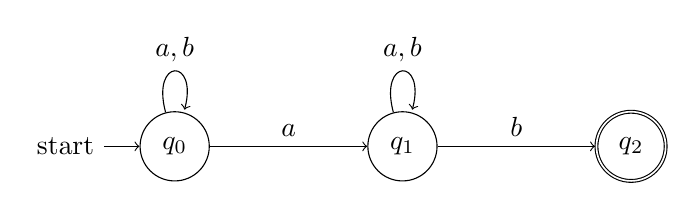
\begin{tikzpicture}[node distance=20 mm]
    \node [state,initial] (0) {$q_0$};
    \node [state] (1) [right=of 0] {$q_1$};
    \node [state,accepting] (2) [right=of 1] {$q_2$};
    \path[->]
        (0) edge [loop above] node [align=center] {$a,b$} (0)
        (0) edge [above] node [align=center] {$a$} (1)
        (1) edge [loop above] node [align=center] {$a,b$} (1)
        (1) edge [above] node [align=center] {$b$} (2);
\end{tikzpicture}\\
\textbf{DFA}\\
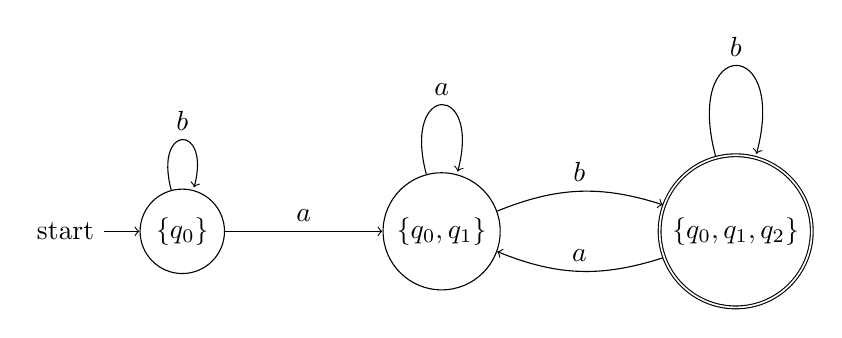
\begin{tikzpicture}[node distance=20 mm]
    \node [state,initial] (0) {$\{q_0\}$};
    \node [state] (1) [right=of 0] {$\{q_0,q_1\}$};
    \node [state,accepting] (2) [right=of 1] {$\{q_0,q_1,q_2\}$};
    \path[->]
        (0) edge [loop above] node [align=center] {$b$} (0)
        (0) edge [above] node [align=center] {$a$} (1)
        (1) edge [loop above] node [align=center] {$a$} (1)
        (1) edge [bend left=20] [above] node [align=center] {$b$} (2)
        (2) edge [bend left=20] [above] node [align=center] {$a$} (1)
        (2) edge [loop above] node [align=center] {$b$} (2);
\end{tikzpicture}
\subsection{Regular Expression to NFA/DFA}
\subsubsection{Regular Expression to NFA}
Suppose $A$ is a language over an alphabet $\Sigma$. If there is a regular expression $R$ where $L(R)=A$, then there is a NFA $N$ such that $L(N)=A$.\\
\newline
We can use the NFA constructions for the concatenation and kleene star as shown in the previous sections.\\
\newpage
\subsubsection{DFA to Regular Expression}
Suppose $A$ is a language over an alphabet $\Sigma$. If there is a DFA $M$ such that $L(M)=A$, then there is a regular expression $R$ such that $L(R)=A$.\\
\begin{enumerate}
    \item Add a new start state with $\epsilon$ arrow to old start state
    \item Add new accept state with $\epsilon$ arrow from old accept states. Make old accept states non-accept.
    \item Remove one (of the old) states at a time: modify regular expressions on arrows that went through the removed state to restore language recognized by machine
\end{enumerate}
\section{Pumping Lemma}
\label{sec:pumpLemma}
\subsection{Countability}
\begin{tabular}{c|c}
    Set & Cardinality \\
    \hline
    $\{0,1\}$ & 2\\
    $\{0,1\}^*$& Countably Infinite\\
    $\mathcal{P}(\{0,1\})$&4\\
    All languages over $\{0,1\}$ ($\mathcal{P}(\{0,1\}^*)$)&Uncountable\\
    Set of all regular expressions over $\{0,1\}$&Countably Infinite\\
    Set of all regular labguages over $\{0,1\}$&Countably Infinite
\end{tabular}\\
\textit{Note: The power set of a countably infinite set is uncountable}
\subsection{Pumping Lemma Definition}
If $A$ is a regular language, then there is a number $p$ (a pumping length) where, if $s$ is any string in $A$ of length at least $p$, then $s$ may be divided into three pieces $s=xyz$ such that
\begin{itemize}
    \item $\vert y\vert>0$
    \item for each $i\geq 0,xy^iz\in A$
    \item $\vert xy\vert\leq p$
\end{itemize}
\textbf{Example:} A pumping length for $A=\{0,1\}^*$ is $p=5$\\
$S\in A$ with $\vert S\vert\geq5$\\
$x=\epsilon$\hspace*{0.5in}$y=S_1$ (the first character in S)\hspace*{0.5in}$z$ is the rest of $S$\\
$xy^iz\in\{0,1\}^*$ for all $i\geq0$
\section{Proving Nonregularity}
\label{sec:proveNonregular}
\textit{The pumping lemma can't be used to prove that a language is regular, but it can be used to prove that a language is not regular}\\
\textbf{Proof Strategy} to show that a language $L$ is not regular
\begin{itemize}
    \item Consider an arbitrary positive integer $p$
    \item Prove that $p$ is not a pumping length for $L$
    \item Conclude that $L$ does not have any pumping lengthand therefore is not regular
\end{itemize}
\subsection{Examples}
\begin{enumerate}
    \item $\Sigma=\{0,1\},L=\{0^n1^n\vert n\geq0\}$\\
    Pick $s=0^p1^p$\\
    Suppose $s=xyz$ with $\vert xy\vert\leq p$ and $\vert y\vert>0$ where $x=0^k,y=0^r,z=0^{p-k-r}1^p$\\
    When $i=0,xy^iz=0^k0^{p-k-r}1^p$ which is not apart of the language and therefore $L$ doesn't have a pumping length.
    \item $\Sigma=\{0,1\},L=\{0^j1^k\vert j\geq k\geq0\}$\\
    Suppose $s=xyz$ with $\vert xy\vert\leq p$ and $\vert y\vert>0$ where $x=0^k,y=0^r,z=0^{p-k-r}1^p$\\
    When $i=0,xy^iz=0^k0^{p-k-r}1^p$ which is not apart of the language since less 0s than 1s and therefore $L$ doesn't have a pumping length.
\end{enumerate}
\section{Pushdown Automata}
\label{sec:pushdown}
A pushdown automata is like an NFA with access to a stack. At each step transition to new state, read the top of the stack, and possibly push or pop a letter from the stack.
\subsection{Definition}
A PDA is specified by a 6-tuple $(Q,\Sigma,\Gamma,\delta,q_0,F)$\\
\begin{itemize}
    \item $Q$ is the finite set of states
    \item $\Sigma$ is the input alphabet
    \item $\Gamma$ is the stack alphabet
    \item $\delta:Q\times\Sigma_\epsilon\times\Gamma_\epsilon\rightarrow\mathcal{P}(Q\times\Gamma_\epsilon)$ is the transition function
    \item $q_0\in Q$ is the start state
    \item $F\subseteq Q$ is the set of accept states
\end{itemize}
\textbf{Transition Label For PDA}\\
input character to read or $\epsilon$, top character of the stack to pop or $\epsilon$, what character to push on top of the stack or $\epsilon$
\subsection{Examples}
\begin{enumerate}
    \item Language: $\{0^n1^{2n}\vert n\geq0\}$\\
    \textbf{PDA:} $(\{q_0,q_1,q_2,q_3,q_4\},\{0,1\},\{\$,\#\},\delta,q_0,\{q_4\})$\\
    $\delta\hspace*{1in}$\begin{tabular}{c|c}
        input & output \\
        \hline
        $(q_0,0,\$)$ & $\emptyset$\\
        $\vdots$ & $\vdots$\\
        $(q_0,\epsilon,\epsilon)$ & $\{(q_1,\$)\}$\\
        $\vdots$ & $\vdots$
    \end{tabular}\\
    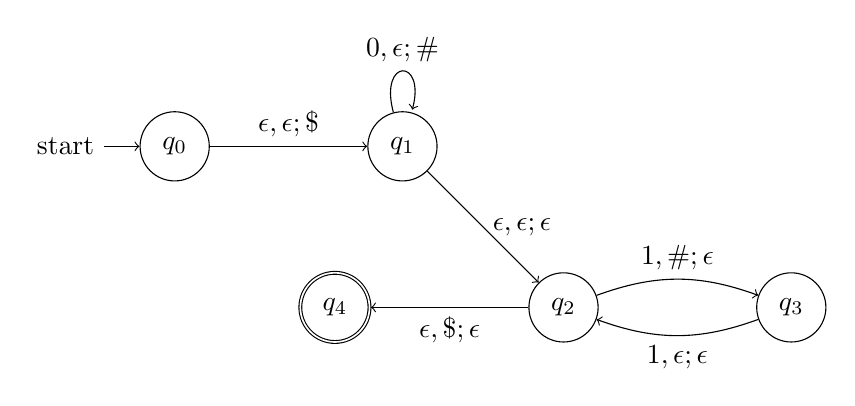
\begin{tikzpicture}[node distance=20 mm]
        \node[state,initial] (0) {$q_0$};
        \node [state] (1) [right=of 0] {$q_1$};
        \node [state] (2) [below right=of 1] {$q_2$};
        \node [state] (3) [right=of 2] {$q_3$};
        \node [state,accepting] (4) [left=of 2] {$q_4$};
        \path[->]
            (0) edge [above] node [align=center] {$\epsilon,\epsilon;\$$} (1)
            (1) edge [loop above] node [align=center] {$0,\epsilon;\#$} (1)
            (1) edge [right] node [align=center] {$\epsilon,\epsilon;\epsilon$} (2)
            (2) edge [bend left=20] [above] node [align=center] {$1,\#;\epsilon$} (3)
            (3) edge [bend left=20] [below] node [align=center] {$1,\epsilon;\epsilon$} (2)
            (2) edge [below] node [align=center] {$\epsilon,\$;\epsilon$} (4);
    \end{tikzpicture}
    \newpage
    \item Language: $\{1^n0^n1^m\vert n,m\geq0\}\cup\{1^n0^m1^n\vert n,m\geq 0\}$\\
    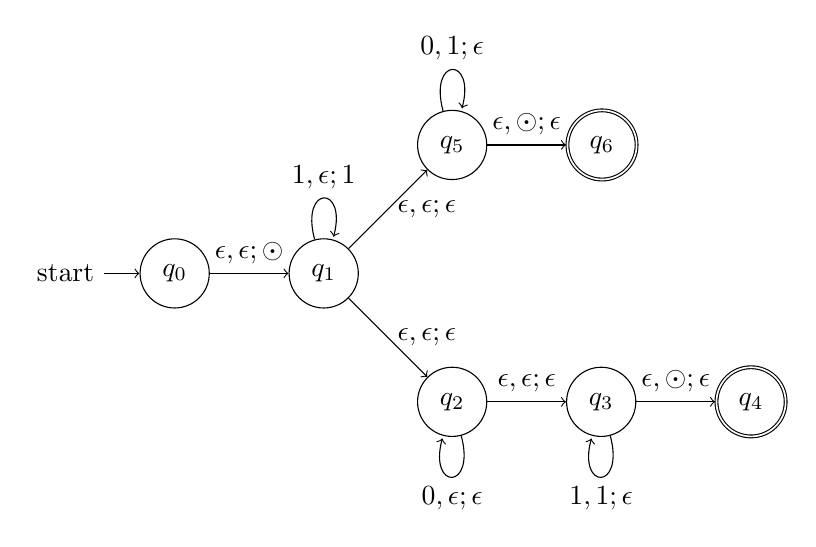
\begin{tikzpicture}
        \node [state,initial] (0) {$q_0$};
        \node [state] (1) [right=of 0] {$q_1$};
        \node [state] (2) [below right=of 1] {$q_2$};
        \node [state] (3) [right=of 2] {$q_3$};
        \node [state,accepting] (4) [right=of 3] {$q_4$};
        \node [state] (5) [above right=of 1] {$q_5$};
        \node [state,accepting] (6) [right=of 5] {$q_6$};
        \path[->]
            (0) edge [above] node [align=center] {$\epsilon,\epsilon;\odot$} (1)
            (1) edge [loop above] node [align=center] {$1,\epsilon;1$} (1)
            (1) edge [right] node [align=center] {$\epsilon,\epsilon;\epsilon$} (5)
            (1) edge [right] node [align=center] {$\epsilon,\epsilon;\epsilon$} (2)
            (2) edge [loop below] node [align=center] {$0,\epsilon;\epsilon$} (2)
            (5) edge [loop above] node [align=center] {$0,1;\epsilon$} (5)
            (5) edge [above] node [align=center] {$\epsilon,\odot;\epsilon$} (6)
            (2) edge [above] node [align=center] {$\epsilon,\epsilon;\epsilon$} (3)
            (3) edge [loop below] node [align=center] {$1,1;\epsilon$} (3)
            (3) edge [above] node [align=center] {$\epsilon,\odot;\epsilon$} (4);
    \end{tikzpicture}
\end{enumerate}
\textit{For each language $L$ over $\Sigma$, there is an NFA $N$ with $L(N)=L$ then there is a PDA $M$ with $L(M)=L$}
\section{Context-free Grammars and Languages}
\label{sec:contextFree}
\subsection{Context-free Grammar}
$G=(V,\Sigma,R,S)$
\begin{itemize}
    \item $V$ is a finite set of symbols that represent phases in the production pattern
    \item $\Sigma$ is the alphabet of symbols of strings generated by CFG
    \item $R$ is the set of rules 
    \item $S$ is the start variable
\end{itemize}
\textbf{Example:} $G_1=(\{s\},\{0\},R,S)$ with rules
\begin{center}
    $S\rightarrow0S$\\
    $S\rightarrow0$
\end{center}
$L(G_1)=0^+$
\subsection{Context-free Language}
A language that is generated by some context-free grammar is a context-free language.\\
\newline
A language is generated by some context-free grammar if and only if it is recognizable by some push-down automaton.\\
\newlinw
\textbf{Every Regular Language is Context Free}
\newpage
\section{Language Closure}
\label{sec:langClose}
\begin{tabular}{c|c}
   True/False  & Closure Claim \\
   \hline
    True & The class of regular languages over $\Sigma$ is closed under complementation\\
    True & The class of regular languages over $\Sigma$ is closed under union\\
    True & The class of regular languages over $\Sigma$ is closed under intersection\\
    True & The class of regular languages over $\Sigma$ is closed under concatenation\\
    True & The class of regular languages over $\Sigma$ is closed under Kleene star\\
    True & The class of non-regular languages over $\Sigma$ is closed under complementation\\
    False & The class of non-regular languages over $\Sigma$ is closed under union\\
    False & The class of non-regular languages over $\Sigma$ is closed under intersection\\
    Flase & The class of non-regular languages over $\Sigma$ is closed under concatenation\\
    False & The class of non-regular languages over $\Sigma$ is closed under Kleene star\\
    False & The class of context-free languages over $\Sigma$ is closed under complementation\\
    True & The class of context-free languages over $\Sigma$ is closed under union\\
    False & The class of context-free languages over $\Sigma$ is closed under intersection\\
    True & The class of context-free languages over $\Sigma$ is closed un concatenation\\
    True & The class of context-free languages over $\Sigma$ is closed under Kleene star
\end{tabular}
\section{Turing Machines}
\label{sec:turing}
\subsection{Definition}
The \textbf{formal definition} of a Turing Machine is $M=(Q,\Sigma,\Gamma,\delta,q_0,q_{accept},q_{reject})$
\begin{itemize}
    \item \textbf{Set of states} $Q$
    \item The \textbf{tape alphabet} $\Gamma$ with $\textvisiblespace\in\Gamma$ and $\Sigma\subseteq\Gamma$. The blank symbol $\textvisiblespace\notin\Sigma$ and the input string is written on the $|w|$-many leftmost cells of tape where the rest of cells have the blank symbol.
    \item The \textbf{transition function} $\delta:Q\times\Gamma\rightarrow Q\times\Gamma\times\{L,R\}$ gives the next state and moves the tape left or right based on the current state and symbol being read at the tape head
    \item The \textbf{start state} $q_0$ is an element of $Q$. Each computation starts at this state
    \item The computation \textbf{halts} when the machine enters an \textbf{accept} ($q_{accept}$) or \textbf{reject} ($q_{reject}$) state
\end{itemize}
\subsection{Example}
\begin{multicols}{2}
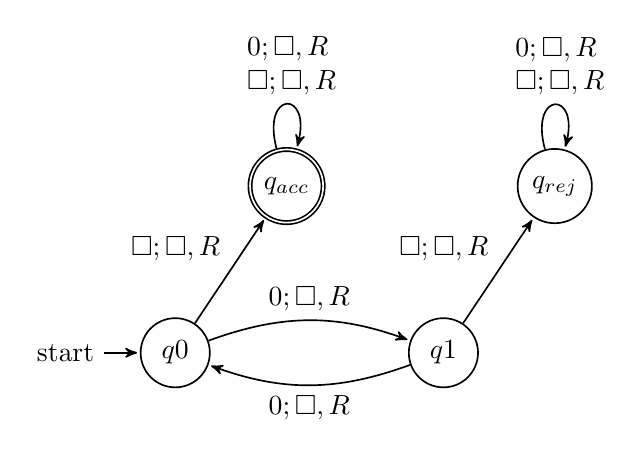
\begin{tikzpicture}[->,>=stealth',shorten >=1pt, auto, node distance=2cm, semithick]
  \tikzstyle{every state}=[text=black, fill=none]
  
  \node[initial,state] (q0)          {$q0$};
  \node[state]         (q1) [right of=q0, xshift=40pt] {$q1$};
  \node[state,accepting]         (qacc) [above right of=q0, yshift=20pt] {$q_{acc}$};
  \node[state]         (qrej) [above right of=q1,yshift=20pt] {$q_{rej}$};
  
  \path (q0) edge [bend left=0] node {$\square; \square, R$} (qacc)
      (q0) edge  [bend left=20] node {$0; \square, R$} (q1)
      (q1) edge [bend left=20] node {$0; \square, R$} (q0)
      (q1) edge [bend left=0] node {$\square; \square, R$} (qrej)
      (qacc) edge  [loop above] node {\parbox{1cm}{$0; \square, R$\newline $\square; \square, R$}} (qacc)
      (qrej) edge  [loop above] node {\parbox{1cm}{$0; \square, R$\newline $\square; \square, R$}}  (qrej)
  ;
\end{tikzpicture}
\columnbreak

Formal definition:$(\{q_0q_1,q_{acc},q_{rej}\},\{0\},\{\textvisiblespace,0\},q_0,q_{acc},q_{rej})$

Sample computation: $w=000$

\begin{tabular}{|c|c|c|c|c|c|c|}
\hline
\multicolumn{1}{|c}{$q0\downarrow$} &  \multicolumn{6}{c|}{\phantom{A}}\\
\hline
$0$ & $0$  & $0$ & $\textvisiblespace $& $\textvisiblespace $& $\textvisiblespace $&  $\textvisiblespace $\\
\hline
\multicolumn{1}{|c}{\phantom{A}}&\multicolumn{1}{c}{$q1\downarrow$} &  \multicolumn{5}{c|}{\phantom{A}}\\
\hline
$\textvisiblespace$ & $0$ & $0$ & $\textvisiblespace$ & $\textvisiblespace$& $\textvisiblespace$ & $\textvisiblespace$ \\
\hline
\multicolumn{2}{|c}{\phantom{A}}&\multicolumn{1}{c}{$q0\downarrow$} &  \multicolumn{4}{c|}{\phantom{A}}\\
\hline
$\textvisiblespace$ & $\textvisiblespace$ & $0$ & $\textvisiblespace$ & $\textvisiblespace$ & $\textvisiblespace$&$\textvisiblespace$ \\
\hline
\multicolumn{3}{|c}{\phantom{A}}&\multicolumn{1}{c}{$q1\downarrow$} &  \multicolumn{3}{c|}{\phantom{A}}\\
\hline
$\textvisiblespace$ & $\textvisiblespace$ & $\textvisiblespace$ & $\textvisiblespace$ & $\textvisiblespace$ & $\textvisiblespace$&$\textvisiblespace$ \\
\hline
\multicolumn{4}{|c}{\phantom{A}}&\multicolumn{1}{c}{$q_{rej}\downarrow$} &  \multicolumn{2}{c|}{\phantom{A}}\\
\hline
$\textvisiblespace$ & $\textvisiblespace$ & $\textvisiblespace$ & $\textvisiblespace$ & $\textvisiblespace$ & $\textvisiblespace$&$\textvisiblespace$ \\
\hline
\end{tabular}
\end{multicols}
\vfill

The language recognized by this machine is $\{0^{2i}\vert i\geq0\}$\\
The labels on the diagram consist of three values \textit{tape symbol being scanned};\textit{tape symbol to write at location of read/write head},\textit{direction to move read/write head}\\
An example definition for one of the transtions using the transition function is $\delta((q_0,\textvisiblespace))=(q_{acc},\textvisiblespace,R)$
\newpage
\subsection{Describing Turing Machines}
\begin{itemize}
\item {\bf Formal definition}: the $7$-tuple of parameters including set of states, 
input alphabet, tape alphabet, transition function, start state, accept state, and reject state; or,
\item {\bf Implementation-level definition}: English prose that describes the Turing machine head 
movements relative to contents of tape, and conditions for accepting / rejecting based on those contents.
\item {\bf High-level description}: description of algorithm (precise sequence of instructions), 
without implementation details of machine. As part of this description, can ``call" and run 
another TM as a subroutine.
\end{itemize}
\section{Recognizable and Decidable Languages}
\subsection{Definition}
\label{sec:decide}
\begin{itemize}
    \item A language $L$ is \textbf{recognized by} a Turing Machine $M$ means $L=\{w\vert M\text{ accepts }w\}$. For each string not in the language, $M$ either rejects or doesn't halt
    \item A language $L$ is \textbf{decided by} a Turing Machine $M$ means $M$ is a decider (halts on each computation) and $M$ recognizes $L$
\end{itemize}
\subsection{Closure}
\begin{itemize}
    \item A {\bf Turing-recognizable} language is a set of strings that 
is the language recognized by some Turing machine. We also 
say that such languages are recognizable.
    \item A {\bf Turing-decidable} language is a set of strings that 
is the language recognized by some decider. We also 
say that such languages are decidable.
    \item An {\bf unrecognizable} language is a language that is not Turing-recognizable.
    \item An {\bf undecidable} language is a language that is not Turing-decidable.
\end{itemize}
\begin{tabular}{c|c}
    True/False & Statement \\
    \hline
    True & Any  decidable language  is  also  recognizable.\\
    False & Any  recognizable language  is  also  decidable.\\
    False & Any  undecidable language  is  also  unrecognizable.\\
    True & Any  unrecognizable language  is  also  undecidable.
\end{tabular}
\section{General Constructions with Turing Machines}
\label{sec:general}
\subsection{Co-Recognizable}
Definition: A language $L$ over an  alphabet $\Sigma$ is called {\bf co-recognizable} if its complement,  defined
as $\Sigma^* \setminus L  = \{ x  \in  \Sigma^* \mid x \notin  L \}$, is Turing-recognizable.\\
\newline
A  language is Turing-decidable if and only if both  it and its complement are Turing-recognizable.\\
\newline
\textbf{Proof, first direction:} Suppose a language $L$ is Turing-decidable. WTS that both it and its complement are Turing-recognizable\\
By definition we have a TM $M$ that decides $L$; namely for each string $W$, $W\in L$, $M$ accepts $W$ and if $W\notin L$, $M$ rejects $W$
\begin{enumerate}
    \item Build a TM that recognizes $L$\\
    We can use $M$ as it is
    \item Build a TM that recognized $\bar L$\\
    We can swap the accept and reject stated in $M$
\end{enumerate}
\textit{We will need to use dovetailing to prove the other direction}
\subsection{Dovetailing}
\textbf{Dovetailing} involves interleaving progress on multiple computations by limiting the number of steps each computation makes in each round\\
\textbf{Proof, second direction:} \\
By definition, we have a TM $M_L$ with $L(M_L)=L$ and another TM $M_C$ with $L(M_C)=\bar L$\\
Build $M_{new}=$``On input $w$
\begin{enumerate}
    \item For $n=1,2,3,\dots$
    \item \hspace*{0.25in} Run $M_L$ on $w$ for at most $n$ steps
    \item \hspace*{0.25in} Run $M_c$ on $w$ for at most $n$ steps
    \item \hspace*{0.25in} If $M_L$ accepts $w$ within $n$ steps, accept
    \item \hspace*{0.25in} If $M_c$ accepts $w$ within $n$ steps, reject
    \item \hspace*{0.25in} increment $n$ and continue loop''
\end{enumerate}
It's sufficient to prove that each string in $L$ is accepted by $M_{new}$ and each string not in $L$ is rejected by $M_{new}$. First let $W$ be an arbitrary string in $L$. By assumption that $M_L$ recognizes $L$, we know that $M_L$ accepts $W$. Let $d$ be the number of steps it takes $M_L$ to halt and accept $W$. By assumption that $M_C$ recognizes $\bar L$, we know that $M_C$ does not accept $W$. We trace the computation of $M_{new}$ on $W$: For all iterations of the loop with $n<d$, step 2 and 3 run for at most $n$ steps and the conditions in step 4 and step 5 are not satisfied. At the loop iteration with $n=d$, the subroutine in step 2 ends with $M_L$ accepting $W$. After the at most $d$ steps of the computation simulated in step 3, in step 4, the condition of the conditional is true, so $M_{new}$ accepts $W$.\\
Next let $W$ be an arbitrary string not in $L$. By assumption that $M_C$ recognizes $\bar L$, we know that $M_C$ accpets $W$. Let $d$ be the number of steps it took $M_C$ to halt and accept $W$. By assumption that $M_L$ recognizes $L$, we know that $M_L$ does not accept $W$. Tracing the computation of $M_{new}$ on $W$ (like before) by definition of $d$, the computation doesn't halt for loop iterations with $n<d$; and at $n=d$ the subroutine in step 2 doesn't halt and accept but in step3 it does so the condition in step 4 isn't satisfied and the computation continues to step 5 where the condition is satisfied and $M_new$ rejects $W$.
\subsection{Union of Turing Decidable Languages}
\textbf{Claim:} If two languages (over a fixed alphabet $\Sigma$) are Turing-decidable, then their union is as well\\
\textbf{Example:} Let $L_1$, $L_2$ be arbitrary decidable languages.\\
Let $M_1,M_2$ be deciders with $L(M_1)=L_1$ and $L(M_2)=L_2$ guaranteed to exist by definition of $L_1$ and $L_2$ being decidable\\
Define $M=$``On input $w$
\begin{enumerate}
    \item Run $M_1$ on $w$
    \item If $M_1$ accepts $w$, accept
    \item otherwise run $M_2$ on $w$
    \item If $M_2$ accepts $w$, accept
    \item Otherwise, reject''
\end{enumerate}
\newpage
\subsection{Intersection of Turing Recognizable Languages}
{\bf Claim}: If two languages  (over a fixed alphabet  $\Sigma$) are Turing-recognizable, then  their union  is  as well.
{\bf Example}: Let $L_1,L_2$ be arbitrary recognizable languages. Let $M_1,M_2$ be TMs with $L(M_1)=L_1$ and $L(M_2)=L_2$ guaranteed to exist by definition of $L_1,L_2$ being recognizable. Goal is to build a TM for $L_1\cup L_2$ (use dovetailing).\\
Define $M=$``On input $w$
\begin{enumerate}
    \item For $n=1,2,\dots$
    \item \hspace*{0.25in} For $M_1$ on $w$ for (at most) $n$ steps
    \item \hspace*{0.25in} If $M_1$ accepts $w$, accept
    \item \hspace*{0.25in} Otherwise, run $M_2$ on $w$ for (at most) $n$ steps
    \item \hspace*{0.25in} If $M_2$ accepts $w$, accpets
    \item \hspace*{0.25in} Otherwise, continue to next loop iteration
\end{enumerate}
\section{Computational Problems}
\label{sec:problems}
A \textbf{computational problem} is decidable iff language encoding its positive problem instances is decidable
\begin{center}
    \begin{tabular}{|lcl|}
    \hline
    \multicolumn{3}{|l|}{{\bf  Acceptance problem} } \\
    & & \\
    \ldots for DFA & $A_{DFA}$ & $\{ \langle B,w \rangle \mid  \text{$B$ is a  DFA that accepts input 
    string $w$}\}$ \\
    \ldots for NFA & $A_{NFA}$ & $\{ \langle B,w \rangle \mid  \text{$B$ is a  NFA that accepts input 
    string $w$}\}$ \\
    \ldots for regular expressions & $A_{REX}$ & $\{ \langle R,w \rangle \mid  \text{$R$ is a  regular
    expression that generates input string $w$}\}$ \\
    \ldots for CFG & $A_{CFG}$ & $\{ \langle G,w \rangle \mid  \text{$G$ is a context-free grammar 
    that generates input string $w$}\}$ \\
    \ldots for PDA & $A_{PDA}$ & $\{ \langle B,w \rangle \mid  \text{$B$ is a PDA that accepts input string $w$}\}$ \\
    & & \\
    \hline
    \multicolumn{3}{|l|}{{\bf Language emptiness  testing} } \\
    & & \\
    \ldots for DFA & $E_{DFA}$ & $\{ \langle A \rangle \mid  \text{$A$ is a  DFA and  $L(A) = \emptyset$\}}$ \\
    \ldots for NFA & $E_{NFA}$ & $\{ \langle A\rangle \mid  \text{$A$ is a NFA and  $L(A) = \emptyset$\}}$ \\
    \ldots for regular expressions & $E_{REX}$ & $\{ \langle R \rangle \mid  \text{$R$ is a  regular
    expression and  $L(R) = \emptyset$\}}$ \\
    \ldots for CFG & $E_{CFG}$ & $\{ \langle G \rangle \mid  \text{$G$ is a context-free grammar 
    and  $L(G) = \emptyset$\}}$ \\
    \ldots for PDA & $E_{PDA}$ & $\{ \langle A \rangle \mid  \text{$A$ is a PDA and  $L(A) = \emptyset$\}}$ \\
    & & \\
    \hline
    \multicolumn{3}{|l|}{{\bf Language equality testing} } \\
    & & \\
    \ldots for DFA & $EQ_{DFA}$ & $\{ \langle A, B \rangle \mid  \text{$A$ and $B$ are DFAs and  $L(A) =L(B)$\}}$\\
    \ldots for NFA & $EQ_{NFA}$ & $\{ \langle A, B \rangle \mid  \text{$A$ and $B$ are NFAs and  $L(A) =L(B)$\}}$\\
    \ldots for regular expressions & $EQ_{REX}$ & $\{ \langle R, R' \rangle \mid  \text{$R$ and $R'$ are regular
    expressions and  $L(R) =L(R')$\}}$\\
    \ldots for CFG & $EQ_{CFG}$ & $\{ \langle G, G' \rangle \mid  \text{$G$ and $G'$ are CFGs and  $L(G) =L(G')$\}}$ \\
    \ldots for PDA & $EQ_{PDA}$ & $\{ \langle A, B \rangle \mid  \text{$A$ and $B$ are PDAs and  $L(A) =L(B)$\}}$ \\
    \hline
    \end{tabular}
    \end{center}
    \newpage
    \subsection{$A_{TM}$ Examples}
    \subsubsection{$A_{TM}$ is Turing-recognizable}
    Define $R_{ATM}=$``On input $x$
    \begin{enumerate}
        \item Type check whether $x=\langle M,w \rangle$ where $M$ is a $TM$ and $w$ string. If not, reject
        \item Run $M$ on $w$
        \item If $M$ accepts $w$, accept
        \item If $M$ rejects $w$, reject
    \end{enumerate}
    WTS $L(R_{ATM})=A_{TM}$\\
    Take an arbitrary $x$
    \begin{enumerate}
        \item if $x\neq\langle M,w\rangle$ for any TM $M$ string $w$. By definition of $A_{TM}$, $x\notin A_{TM}$ and tracing $R_{ATM}$ on $x$ rejects in type check of $x$, so $R_{ATM}$ doesn't accept $x$
        \item $x=\langle M,q\rangle$
        \begin{enumerate}
            \item $w\in L(M)$\\
            By def of $A_{TM}$, $x\in A_{TM}$ and tracing $R_{ATM}$, $x$ passes type check and $R_{ATM}$ runs $M$ on $w$ as a subroutine. The subroutine halts and accepts, so $R_{ATM}$ accepts $x$
            \item $w\notin L(M)$
            \begin{enumerate}
                \item $M$ rejects $w$\\
                By def of $A_{TM}$, $x\notin A_{TM}$ and tracing $R_{ATM}$, $x$ passes type check and $R_{ATM}$ runs $M$ on $w$ as a subroutine. The subroutine halts and rejects, so $R_{ATM}$ rejects $x$
                \item $M$ loops on $w$\\
                By def of $A_{TM}$, $x\notin A_{TM}$ and tracing $R_{ATM}$, $x$ passes type check and $R_{ATM}$ runs $M$ on $w$ as a subroutine. The subroutine doesn't halt so $R_{ATM}$ doesn't halt on $x$, so it doesn't accept $x$
            \end{enumerate}
        \end{enumerate}
    \end{enumerate}
    \subsubsection{Other $A_{TM}$ properties}
    \begin{itemize}
        \item $A_{TM}$ is not decidable
        \item $\bar{A_{TM}}$ is not recognizable
        \item $\bar{A_{TM}}$ is not decidable
    \end{itemize}
    \section{Computable Functions and Mapping Reduction}
    \label{sec:reduction}
    For any languages $A$ and $B$, $A$ is  {\bf  mapping  reducible to} $B$  means there is a computable function 
    $f : \Sigma^* \to \Sigma^*$ such that {\it for all} strings  $x$ in $\Sigma^*$, 
    \[
    x  \in  A \qquad \qquad \text{if and  only  if} \qquad \qquad f(x) \in B.
    \]
    Notation:  when $A$  is mapping reducible to $B$, we write $A  \leq_m B$.\\
    {\it Intuition:} $A \leq_m B$ means $A$ is no harder than $B$, i.e. that the level 
    of difficulty of $A$ is less than or equal the level of difficulty of $B$.\\
    \newline
    A function $f: \Sigma^* \to \Sigma^*$ is a {\bf computable function} means there is some Turing machine such that, 
for each $x$, on input $x$ the Turing machine halts with exactly $f(x)$ followed by all blanks on the tape
    \subsection{Mapping Reduction Decidability}
    \begin{itemize}
        \item  If $A \leq_m B$ and $B$ is decidable, then $A$ is decidable.
        \item If $A \leq_m B$ and $A$ is undecidable, then $B$ is undecidable.
        \item For any language decidable language $X$ and any 
set $Y$ with at least one string string in $Y$ and at least one string not in $Y$, $X \leq_m Y$, as witnessed by the identity function (one in and one out case)
    \end{itemize}
    \newpage
    \subsection{Halting Problem}
    \[
    HALT_{TM} = \{ \langle M, w \rangle \mid \text{$M$ is a  Turing machine, $w$ is  a string, and $M$ halts on $w$} \}
    \]\\
We know $A_{TM}$ is undecidable. If we could prove that $A_{TM} \leq_m HALT_{TM}$ then we could conclude that $HALT_{TM}$ is undecidable too.\\
Define $F: \Sigma^* \to \Sigma^*$ by
    \[
    F(x) =  \begin{cases}
    const_{out} \qquad &\text{if  $x \neq \langle M,w \rangle$ for any Turing machine  $M$ and string  $w$ over the alphabet of $M$} \\
    \langle M'_x, w \rangle \qquad &  \text{if $x = \langle M, w \rangle$ for some Turing machine  $M$ and string $w$ over the alphabet of $M$.}
    \end{cases}
    \]
    where $const_{out}  =  \langle  
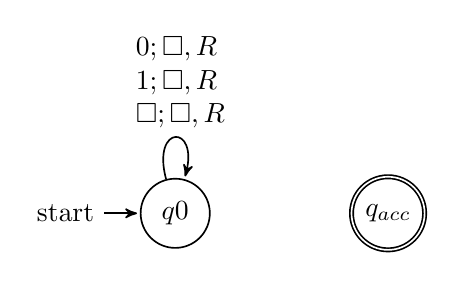
\begin{tikzpicture}[->,>=stealth',shorten >=1pt, auto, node distance=2cm, semithick]
            \tikzstyle{every state}=[text=black, fill=none]
            
            \node[initial,state] (q0)          {$q0$};
            \node[state,accepting]         (qacc) [right of=q0, xshift=20pt] {$q_{acc}$};
            
            \path (q0) edge  [loop above] node {\parbox{1cm}{$0; \square, R$\newline$1; \square, R$\newline $\square; \square, R$}} (q0)
            ;
          \end{tikzpicture},  \varepsilon  \rangle$
    and  $M'_x$ is a Turing machine that computes like $M$ except, if the computation of $M$ ever were to go to a  reject state,
    $M'_x$ loops instead.   




    $F( \langle 
        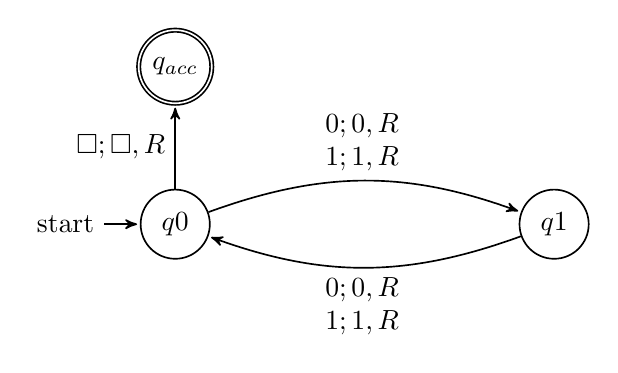
\begin{tikzpicture}[->,>=stealth',shorten >=1pt, auto, node distance=2cm, semithick]
            \tikzstyle{every state}=[text=black, fill=none]
            
            \node[initial,state] (q0)          {$q0$};
            \node[state]         (q1) [right of=q0, xshift=80pt] {$q1$};
            \node[state,accepting]   (qacc) [above of=q0] {$q_{acc}$};
            
            \path (q0) edge [bend left=20] node {\parbox{1cm}{$0; 0,R$\newline $1; 1, R$}} (q1)
                (q1) edge [bend left=20] node {\parbox{1cm}{$0; 0,R$\newline $1; 1, R$}} (q0)
                (q0) edge  [bend left=0] node {$\square; \square, R$} (qacc)
            ;
        \end{tikzpicture}, \varepsilon \rangle)$ = $\langle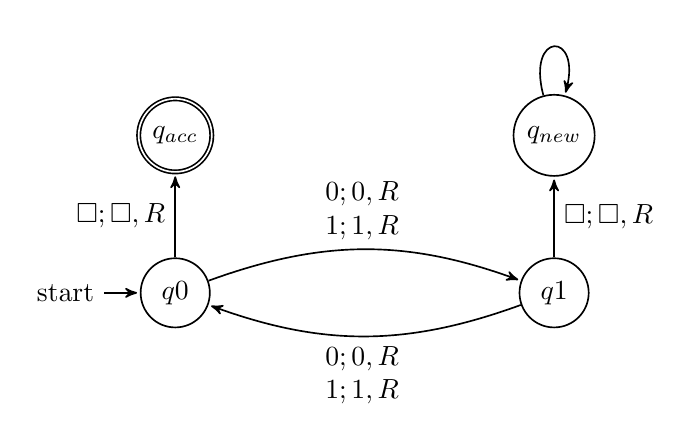
\begin{tikzpicture}[->,>=stealth',shorten >=1pt, auto, node distance=2cm, semithick]
            \tikzstyle{every state}=[text=black, fill=none]
            
            \node[initial,state] (q0)          {$q0$};
            \node[state]         (q1) [right of=q0, xshift=80pt] {$q1$};
            \node[state,accepting]   (qacc) [above of=q0] {$q_{acc}$};
            \node [state] (qnew) [above of=q1] {$q_{new}$};
            
            \path (q0) edge [bend left=20] node {\parbox{1cm}{$0; 0,R$\newline $1; 1, R$}} (q1)
                (q1) edge [bend left=20] node {\parbox{1cm}{$0; 0,R$\newline $1; 1, R$}} (q0)
                (q0) edge  [bend left=0] node {$\square; \square, R$} (qacc)
                (qnew) edge [loop above] node {} (qnew)
                (q1) edge [right] node {$\square; \square, R$} (qnew)
            ;
        \end{tikzpicture},\epsilon \rangle$ 
        \subsection{Mapping Reduction Recognizability}
        \begin{itemize}
            \item If $A \leq_m B$ and $B$ is recognizable, then $A$ is recognizable.
            \item If  $A \leq_m B$ and $A$ is unrecognizable, then $B$ is unrecognizable.
            \item To prove that a recognizable language $R$ is undecidable, prove that $A_{TM} \leq_m R$.
            \item To prove that a co-recognizable language $U$ is undecidable, prove that $\overline{A_{TM}} \leq_m U$,
 i.e. that $A_{TM} \leq_m \overline{U}$.
        \end{itemize}
        \subsection{Computation Decidability Based on Reduction}
        \begin{itemize}
        \item $A_{TM}$ is recognizable, undecidable, and not-co-recognizable.
        \item $\overline{A_{TM}}$ is unrecognizable, undecidable, and co-recognizable.
        \item $HALT_{TM}$ is recognizable, undecidable, and not-co-recognizable.
        \item $\overline{HALT_{TM}}$ is unrecognizable, undecidable, and co-recognizable.
        \item $E_{TM}$ is unrecognizable, undecidable, and co-recognizable.
        \item $\overline{E_{TM}}$ is recognizable, undecidable, and not-co-recognizable.
        \item $EQ_{TM}$ is unrecognizable, undecidable, and not co-recognizable
        \item $\overline{EQ_{TM}}$ is unrecognizable, undecidable, and not co-recognizable
        \end{itemize}
        \newpage
        \section{Other Models of Computation}
        \label{sec:otherModels}
        {\bf  Church-Turing Thesis}: The informal notion of algorithm is formalized completely  and correctly by the 
formal definition of a  Turing machine. In other words: all reasonably expressive models of 
computation are equally expressive with the standard Turing machine.


\begin{center}
{\large \it  Some examples of models that are {\bf equally expressive} with deterministic Turing machines: }
\end{center}
\subsection{May-stay machines }
The May-stay machine model is the same as the usual Turing machine model,  except that
on each transition, the tape head may move L, move R, or Stay. 

Formally: $(Q, \Sigma, \Gamma, \delta, q_0, q_{accept}, q_{reject})$ where 
\[
  \delta: Q \times \Gamma \to Q \times \Gamma \times \{L, R, S\}
\]

{\bf Claim}: Turing machines and May-stay machines are equally expressive. {\it To prove \ldots}

To translate a standard TM to a may-stay machine: never use the direction $S$!


To translate one  of the  may-stay machines to standard TM:
any time TM would Stay, move right  then  left.

\subsection{Multitape Turing machine}
A multitape Turing machine with $k$ tapes can be formally represented as 
$(Q, \Sigma,  \Gamma, \delta, q_0, q_{acc}, q_{rej})$ 
where $Q$ is the finite set of  states,
$\Sigma$ is the  input alphabet with  $\textvisiblespace \notin \Sigma$,
$\Gamma$  is the  tape alphabet with $\Sigma \subsetneq \Gamma$ ,
$\delta: Q\times \Gamma^k\to Q \times \Gamma^k \times \{L,R\}^k$ 
(where $k$ is  the number of  states)


If $M$ is a standard  TM, it is a $1$-tape machine.


To translate a $k$-tape machine  to  a standard TM:
Use a  new symbol to separate the contents of each tape
and keep track of location of  head with  special version of each
tape symbol. 
\end{document}
